\section{Experiment}

The first experiment is focus on the context switching time.
We implemented a simple application under Contiki.
The application contains two indentical tasks.
The tasks wait for 1ms in the foreground and then goes to the background letting the scheduler runs the next task.
The tasks run in an infinite loop.
The source code of the tasks are shown in the listing \ref{lst:simple-task-code}.

\begin{lstlisting}[style=CStyle, label={lst:simple-task-code}, caption={Source code of the simple task implemented in Contiki}]
PROCESS_THREAD(task, ev, data)
{
    PROCESS_BEGIN();

    while (1)
    {
        PROCESS_PAUSE();
        // Wait for 1ms
        clock_delay_usec(1000);
    }

    PROCESS_END();
}
\end{lstlisting}


We choose to use Contiki for this measurement for its cooperative scheduling.
This kind of scheduling allows us to know when a task is in the foreground and when it goes to the background.
With a preemptive scheduling, in the other hand, we don't know when the task is preempted.
This issue is discussed later in our work.

\subsection{Reference measurement}

We need a reference measurement for the context switching time in order to develop this benchmarking framework.
This value would allow us to assess the performance of our framework.
Commonly, the context switching time is measured using an oscilloscope.
We updated our simple task by adding GPIO calls in order for the oscilloscope to detect it.
The task will set up a GPIO, wait for 1ms, and then clear the GPIO.
The source code of the updated task is shown in the listing \ref{lst:gpio-task-code}.
The two tasks use different GPIO in order to differenciate them with the oscilloscope.

\begin{lstlisting}[style=CStyle, label={lst:gpio-task-code}, caption={Source code of the task with GPIO calls}]
  PROCESS_THREAD(task, ev, data)
  {
      PROCESS_BEGIN();
  
      while (1)
      {
          PROCESS_PAUSE();
          // Set the GPIO PC3 up
          GPIO_SET_PIN(GPIO_PORT_TO_BASE(GPIO_C_NUM), GPIO_PIN_MASK(3));
          // Wait for 1ms
          clock_delay_usec(1000);
          // Clear the GPIO PC3
          GPIO_CLR_PIN(GPIO_PORT_TO_BASE(GPIO_C_NUM), GPIO_PIN_MASK(3));
      }
  
      PROCESS_END();
  }
\end{lstlisting}

\paragraph{Measurement setup}

The oscilloscope used for the measurement was the Tektronix MSO 56 available at the Welcome Lab.
We used two channels to measure the voltage of the two GPIOs used by the application.
The measurement is displayed in the figure \ref{fig:measurement-value-wave}.
High value means that the task is running in the foreground.
Low value means that the task is sleeping in the background.

\begin{figure}[!ht]
  \centering
  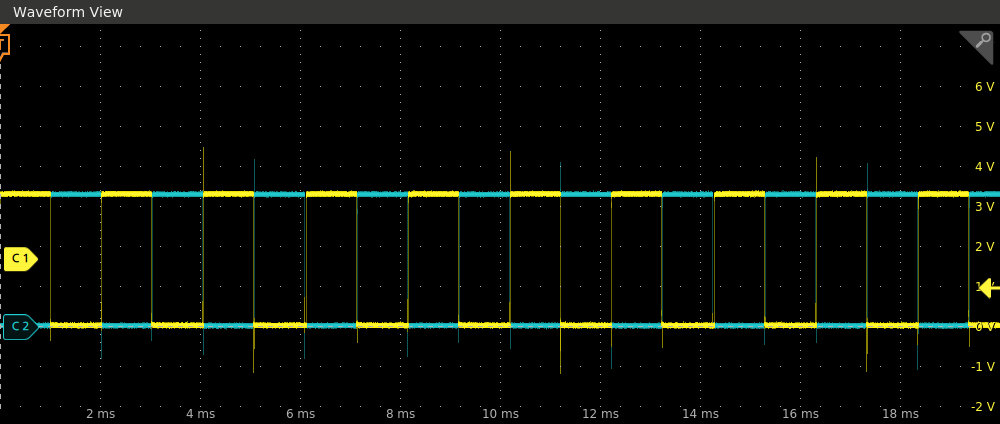
\includegraphics[scale=0.5]{assets/measurement-value-wave.png}
  \caption{\label{fig:measurement-value-wave}Voltage measurement of the two GPIOs; Each color represents a task}
\end{figure}

\paragraph{Measurement value}

The context switching time is the time during which no task is running.
This is visible with the oscilloscope when both channels are low.

With the oscilloscope, we made four measurements.
The first two measurements are the context switching times from task 1 to task 2 and from task 2 to task 1.
The other two measurements are the time taken by the two tasks.
These last measurements should be arround 1ms.
The measurements are shown in the table \ref{tab:reference-measurement}.

With these results, we can see that the duration of both tasks is 1ms with no variation.
We also extract with this measurement our reference value.
From task 1 to task 2, we have 14.68$\mu$s of context switching time and from task 2 to task 1, we have 14.88$\mu$s.
Our benchmarking framework should compute the context switching time of that same application and output a value between 13.30$\mu$s and 16.26$\mu$s for an error bound of 10\%.

\begin{table}[!ht]
  \centering
  \begin{tabular}{llll}
                        & \multicolumn{3}{c}{Time ($\mu$s)}                              \\ \cline{2-4} 
                        & \multicolumn{1}{c}{Mean} & Min   & \multicolumn{1}{c}{Max} \\ \cline{2-4} 
  From task 1 to task 2 & 14.68                    & 13.75 & 15.33                   \\
  From task 2 to task 1 & 14.88                    & 13.93 & 15.77                   \\
  Duration of task 1    & 1003                     & 1003  & 1003                    \\
  Duration of task 2    & 1003                     & 1003  & 1003                   
  \end{tabular}
  \caption{Context switching times and task durations measured with the oscilloscope Tektronix MSO 56}
  \label{tab:reference-measurement}
\end{table}


\subsection{Methodology}

\paragraph{Integration in the kernel}

\paragraph{Minimal impact framework}